\documentclass[a4paper]{article}
\usepackage{hyperref}
\usepackage{microtype}
\usepackage{mathpazo,xcolor}
\usepackage[top=1cm,left=1cm,right=1cm,bottom=1cm]{geometry}
\usepackage{graphicx,soul,lipsum}
\parindent0pt
\makeatletter
\def\HUGE{\@setfontsize\HUGE{65}{90}}
\makeatother
\begin{document}
\thispagestyle{empty}

% define university colors
\definecolor{cprimary}{RGB}{0,39,76}
\definecolor{csecondary}{RGB}{255,112,0}

\newcommand{\name}[1]{\textit{#1}}

\raggedbottom
\begin{minipage}{0.95\textwidth}
\sffamily
\centering
\LARGE{\color{csecondary}\bf GEOMETRY SEMINAR}\\

\Large{\color{cprimary}\textbf{\so{Department of Mathematics}}}\\

\large{\color{cprimary}\textbf{\so{California State University Fullerton}}}\\
\smallskip
\large{\color{cprimary}\textbf{{\color{csecondary}Zoom meeting room:} \href{https://fullerton.zoom.us/j/89343255295?pwd=ZFR3VThaM29ZYkdReGVQS0daS1pHUT09}{893\ 4325\ 5295}\quad {\color{csecondary}Password:} 112358}}
%\large{\color{cprimary}\textbf{\so{Zoom Meeting Room: \ref{https://fullerton.zoom.us/j/89343255295?pwd=ZFR3VThaM29ZYkdReGVQS0daS1pHUT09}{893\ 4325\ 5295}\quad Password: 112358}}}\\

\bigskip

\begin{minipage}[b]{0.47\textwidth}
\normalsize
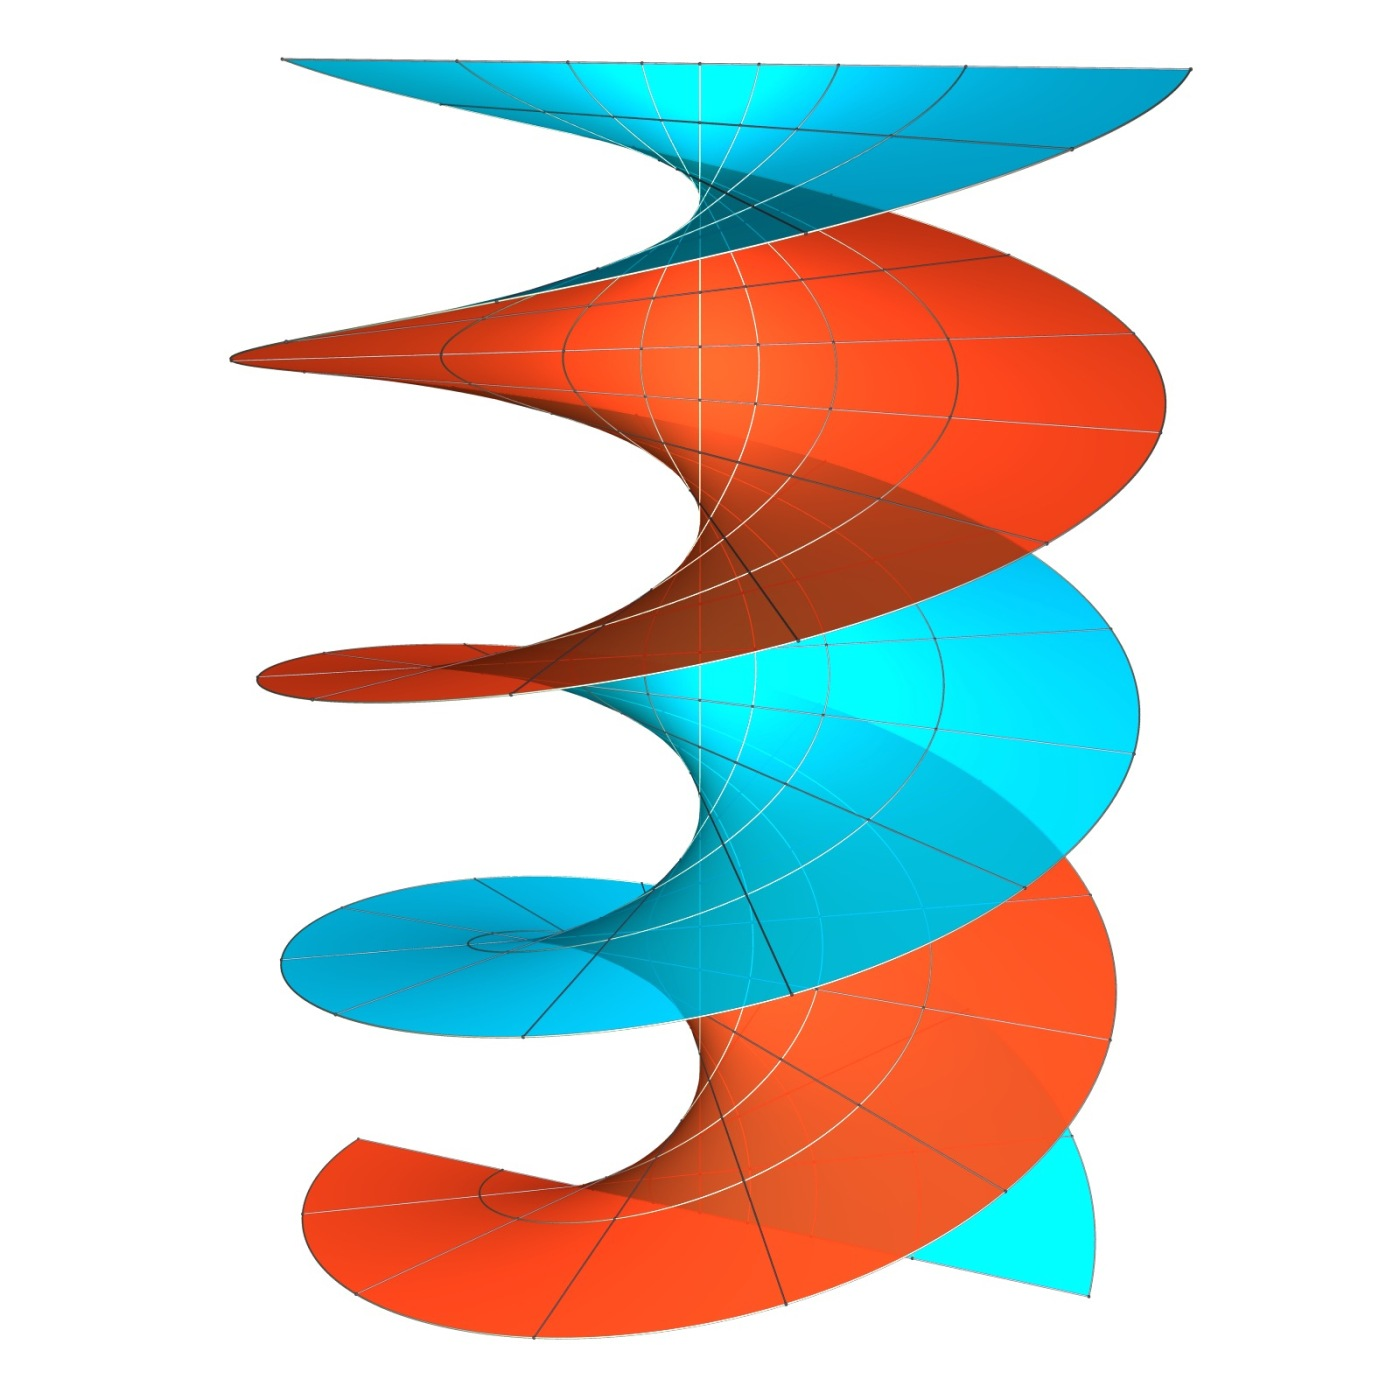
\includegraphics[width=\linewidth,height=3.15in]{helicoid.jpg}
\medskip
\medskip

{\large\raggedright
{\textbf{\color{csecondary}ABOUT THE SEMINAR}}\par
}
\normalsize
\smallskip

The Geometry Seminar at Cal State Fullerton was established in the Spring semester 2007, and the first speakers
were Professors Zhiqin Lu and Ovidiu Munteanu (at that time both from UC Irvine). Since then, the seminar
became the meeting place of faculty interested in Topology- and Geometry-related themes, and their students. We
value very much the students' participation to our events, which we feel should guide our more motivated students
interested to pursue a graduate career, where a good mastery of various topics in Topology and Geometry is
welcome.
\medskip

Many collaborative efforts were born out of the conversations among our participating faculty members. E.g. at the
American Mathematical Society's Meeting 1167, which took place on May 1-2, 2021, the Special Session on
Differential Geometry and Geometric PDE was organized by Professors Alfonso Agnew, Nicholas Brubaker, Thomas
Murphy, Shoo Seto, and Bogdan Suceav\u{a}. Such efforts are the expression of our academic environment and our
collaborating atmosphere.
\medskip
\begin{center}

\includegraphics[width=0.7\linewidth]{csuf_seal.png}
\end{center}
\smallskip

\rule{0pt}{32pt}
\end{minipage}\hspace{5pt}
\begin{minipage}[b]{0.47\textwidth}
\textbf{\color{csecondary}\large SCHEDULED TALKS}\par


{\leavevmode \raggedright
\textbf{\color{cprimary} Friday, February 18, 9:00 am}\\ \name{Simona Nistor}, from University Al. I. Cuza Ia\c{s}i
\textbf{\color{cprimary} Friday, February 25, 9:00 am}\\ \name{Martha Dussan Angulo}, Universidade de S\-{a}o Paolo, Brazil\\
\textbf{\color{cprimary} Friday, March 4, 9:00 am}\\ Oliver Dragi\v{c}evi\'{c}, University of Ljubljana, Slovenia\\
\textbf{\color{cprimary} Friday, March 11, 9:00 am}\\ no event\\
\textbf{\color{cprimary} Friday, March 18, 9:00 am}\\ \name{Vera Toni\'{c}}, University of Rijeka, Croatia\\
\textbf{\color{cprimary} Friday, March 25, 9:00 am}\\ \name{Baisheng Yan}, Michigan State University\\
\textbf{\color{cprimary} Friday, April 1, 9:00 am}\\ no event\\
\textbf{\color{cprimary} Friday, April 8, 9:00 am}\\ 2022 AMS--MAA Joint Mathematical Meetings, (taking place virtually this year)\\
\textbf{\color{cprimary} Friday, April 15, 9:00 am}\\ no event\\
\textbf{\color{cprimary} Friday, April 22, 9:00 am}\\ \name{Nicoleta Voicu}, Transylvania University, Br\d{a}ov, Romania\\
\textbf{\color{cprimary} Friday, April 29, 9:00 am}\\ no event\\
\textbf{\color{cprimary} Friday, May 6, 9:00 am}\\ no event\\
\textbf{\color{cprimary} Friday, May 13, 9:00 am}\\ \name{Thomas Mark}, University of Virginia\\
\par{}
}

\vspace{0.1in}
\medskip

\large{\color{csecondary}\textbf{VENUE}}

The symposium will take place virtually via Zoom.

\medskip

\large{\color{csecondary}\textbf{WEBSITE}}
More information about CSUF's virtual geometry seminar, including an up-to-date calendar with speaker times, information about past and upcoming speakers, and recordings of past talks.\\
Visit our website at\\ \href{https://wcasper.github.io/geometry-seminar/}{https://wcasper.github.io/geometry-seminar/}.

\medskip
\textbf{\color{csecondary}\large 2021-2022 ORGANIZERS}\par
\name{W.~Riley Casper}, CSUF\\
\name{Shoo Seto}, CSUF

\medskip

\textbf{\color{csecondary}\large CONTACT }\par

\name{W.~Riley Casper}, CSUF\\
Email: \href{mailto:wcasper@fullerton.edu}{wcasper@fullerton.edu}

\rule{0pt}{78pt}
\end{minipage}
\vspace*{-70pt}

\end{minipage}
\end{document}

